\documentclass[a4paper]{article}
\newcommand{\CS}{%
   {\fontfamily{ppl}\fontshape{it}\selectfont Code\_Saturne}\xspace}
\usepackage[english]{babel}
\usepackage[T1]{fontenc}
\usepackage[utf8]{inputenc}
\usepackage{amsfonts,amsmath,amssymb,mathrsfs,amsthm}
\usepackage{lmodern}
\usepackage{graphicx}
\usepackage{tikz}
\usepackage{xspace}
\usepackage{hyperref}

\title{Objective A.2: Validation for $Re_\tau = 1020$}

%\author{Your names and group number}
\date{\today}

\begin{document}
\maketitle

%\begin{abstract}
%Enter a short summary here. What topic do you want to investigate and why? What experiment did you perform? What were your main results and conclusion?
%\end{abstract}

\section{Introduction}
The validation procedure for the turbulent channel flow case at $Re_\tau = 1020$ is fully described here. 
The first objective of this validation procedure is to perform a comparison of SGS turbulence models implemented in \CS.
The second one is to define a meshing strategy for the turbulent channel flow.

\section{Geometry}
The geometry used is sketched figure \ref{fig_geom}. $x$ is the streamwise direction, $y$ the wall-normal one and $z$ the spanwise one. The size of the domain is $[6.283, 2, 3.142]$, as was used by M. Bla\v{z} in his PhD. This is similar to the domain used by Abe et al. for a turbulent channel flow at $Re_\tau = 1020$, except \textbf{our domain is halved} in the $\textbf{x}$ and $\textbf{z}$ directions.

\begin{figure}[htbp]
\centering
  \begin{tikzpicture}
    \draw [very thick,->] (0,1.5,0) -- (1.5,1.5,0);
    \draw [very thick,->] (0,1.5,0) -- (0,3,0);
    \draw [very thick,->] (0,1.5,0) -- (0,1.5,1.5);
    \node at (1.375,1.75,0) {$x$};
    \node at (0.25,2.8,0) {$y$};
    \node at (0.25,1.5,1.25) {$z$};
    \foreach \x in{0,9}
    { \foreach \y in{0,3}
    { \foreach \z in{0,6}
    {   \draw (0,\y,\z) -- (9,\y,\z);
        \draw (\x,0,\z) -- (\x ,3,\z);
        \draw (\x,\y,6) -- (\x,\y,0);
    }
    }
    }
  \end{tikzpicture}
\caption{Sketch of the geometry used for the turbulent channel flow LES.}\label{fig_geom}
\end{figure}

\section{Meshes}
The first simulations were based on the mesh provided by M. Bla\v{z}. This allowed us to obtain results quickly, while postponing the pitfall of meshing the domain. As described in the next section, we later build a finer mesh. For those structured hexahedral meshes, the number of cells ($n_i$) and their size ($\Delta_i$) in each direction is:
\begin{tabular}{|c|c|c|}
\hline
    & $n_i$ & $\Delta_i^+$ \\ \hline
$x$ & $160$ / $200$ & $40$ / $32$ \\ \hline
$y$ & $100$ / $172$ & $[2,67]$ / $[1,16]$ \\ \hline
$z$ & $160$ / $200$ & $20$ / $16$ \\ \hline
\end{tabular}

\section{Meshing strategy}
Overall, the first mesh provided was good, except in the wall-normal direction: at the wall, the first cell was judged too large. In addition, in the middle of the channel, the cells have a very large $y$ size compared to $\Delta_z^+$. First, the resolution in $x$ and $z$ was slightly increased by a factor $1.25$. Then, we decided to impose the following in the wall-normal direction:
\begin{itemize}
\item At the wall, the first cell should have $\Delta_y^+ \approx 1$ so the LES is wall-resolved
\item Further away from the wall, the size of the cells should increase according to a geometric serie with a ratio of 1.09 (\CS's BPG indicate the ratio should be below 1.1)
\item The maximum size of the cells in the $y$ direction is equal to the size of the cells in the $z$ direction.
\end{itemize}

Those criterions were used to build a 1D mesh for half the domain with gmsh, as described in appendix \ref{section_gmsh}. \CS preprocessor was then used for $2$ things:
\begin{itemize}
\item Build a 1D mesh of the domain. This requires to apply a combination of symmetry and translation to the initial mesh, and some mesh joining operations.
\item Build a complete 3D mesh of the domain. This requires to apply some looped translations to the 1D mesh, and some joining operations.
\end{itemize}
More recent versions of \CS can extrude a given mesh, so there it is no longer necessary to combine translations and joinings of the 1D mesh.

\section{Case setup}
In this study, the reference distance $D_{ref}$ is the channel half-height, which is $1$. The reference velocity $U_{ref}$ is the bulk velocity, which is also $1$. The density is also set to $1$ while the viscosity is set to $4.826~10^{-5}$ $Pa.s$. The Reynolds number based on those quantities is around $20720$.

An explicit source term in the $x$ momentum conservation equation is driving the turbulent channel flow. The amplitude of this source term is $\left( Re_\tau \nu \right)^2 \approx 0.04923^2$, assuming $Re_\tau = 1020$.

\section{Transitory and steady state}
The velocity is initialised with a parabolic profile combined with white noise. To trigger the transition to turbulence, a rotation source term is introduced during $40~T_{ref}$, with $T_{ref} = D_{ref} / U_{ref}$. This source term is then removed and the simulation is performed for another $360~T_{ref}$ so the flow can reach a fully developed turbulent state. Statistics are then gathered during $2000~T_{ref}$ ($\approx 4$ times longer than in the DNS, but our domain is halved in the $x$ and $z$ directions).

As there is no need for high accuracy during the transient part, higher time steps are often used during the first $80~T_{ref}$, while maintaining a maximal CFL number below $1$. The remaining part of the transient and the collect of the statistics are performed with a time-step halved, thus maintaining the maximal CFL number below $0.5$. For the coarser (finer) mesh, this corresponds to a time-step of $0.005$ ($0.004$) $T_{ref}$.

\section{Numerical configuration}
The version 4.0.4 of \CS was used for the present simulations. A modified version of \verb!cs_time_moment.c! was used to include rev 8550 which fixes time moment weighting when no moment is active at the initial time step. The default options were used. The post-processing of the stress at the boundaries was activated to measure the friction at the wall and the development of the turbulence.

For the collect of statistics, many moments were defined in the subroutine \verb!cs_user_time_moments()!. At the end of the simulation, they are written in EnsightGold binary format as 3D fields. We brewed a bunch of small programs able to read those binary fields, perform spatial averaging and write the result as 1D text files (\verb!.1d.dat!). Those smaller files are analysed by a scilab (\verb!.sce!) script which output the quantities of interest in wall-units inside a \verb!csv! file, that can easily be imported into Microsoft Excel. The main drawback of this method is that EnsightGold Binary files are written in simple precision, thus reducing the precision from 16 to 8 digits.

Our plan is to perform those post-processing operations (space averaging) within \CS because simple precision data may not allow accurate post-processing on very large meshes. As the present mesh is small enough, there is no immediate need for those developments.

\section{Brief description of the SGS models}
We have performed LES with different SGS models. Those models are quickly described here. We assume in this section that:
\begin{eqnarray}
\Omega_i & \mbox{is} & \mbox{the volume of cell } i \nonumber \\
\Delta & \mbox{is} & \mbox{the filter width: } \Delta = 2 \Omega_i^{1/3} \nonumber \\
\mu & \mbox{is} & \mbox{the viscosity} \nonumber \\
\mu_t & \mbox{is} & \mbox{the subgrid scale viscosity} \nonumber \\
\nu & \mbox{is} & \mbox{the kinematic viscosity} \nonumber \\
\nu_t & \mbox{is} & \mbox{the subgrid scale kinematic viscosity} \nonumber \\
u & \mbox{is} & \mbox{the velocity vector} \nonumber \\
U_i^+ & \mbox{is} & \mbox{the averaged velocity in wall units} \nonumber \\
\nabla u & \mbox{is} & \mbox{the velocity gradient tensor} \nonumber \\
S & \mbox{is} & \mbox{its symmetric part: } S = \frac{\nabla u + \left( \nabla u \right)^t }{2} \nonumber \\
R_{ij} & \mbox{is} & \mbox{the Reynolds stress tensor} \nonumber \\
\varepsilon_r & \mbox{is} & \mbox{the resolved dissipation : } \varepsilon_r = \nu \frac{\overline{\partial_k u'_i \partial_k u'_i}}{2} \nonumber \\
\varepsilon_t & \mbox{is} & \mbox{the subgrid scale dissipation : } \varepsilon_t = \frac{\overline{\nu'_t \partial_k u'_i \partial_k u'_i}}{2} \nonumber \\
\varepsilon & \mbox{is} & \mbox{the sum of the resolved and SGS dissipations} \nonumber \\
\end{eqnarray}

\subsection{No model}
We have performed some simulations without specifying a SGS model. Usually, those simulations are performed with \verb!iturb=42! (WALE model) and a modified function \verb!viswal! that imposes a turbulent viscosity equal to zero.

\subsection{Standard Smagorinsky}
This model is selected with \verb!iturb=40!. It leads to:
$$\mu_t = \rho \left( C_s \Delta \right)^2 \sqrt{2 S_{ij} S_{ij}}$$

$C_s$ is the Smagorinsky constant, its default value in \CS is $0.065$.

\subsection{Dynamic Smagorinsky}
This model is selected with \verb!iturb=41!. It is more complex and involves a filter. Assuming the filtered field $f$ is $\widehat{f}$, this model leads to:
\begin{eqnarray}
\mu_t & = & \rho C \Delta^2 \sqrt{2 S_{ij} S_{ij}} \nonumber \\
C & = & \frac{\widehat{M_{ij} L_{ij}}}{\widehat{M_{ij} M_{ij}}}
\end{eqnarray}

The exact expression for $M_{ij}$ and $L_{ij}$ can be found in the literature. When the flow has some homogeneous directions, it is possible to smooth the model using spatial averaging of the numerator and denominator used to obtain $C$. By default in version 4.0, some clippings are applied on $C$ to further stabilize the model:
$$-100 C_s^2 \leq C \leq 100 C_s^2$$

$C_s$ is the Smagorinsky constant, its default value in \CS is $0.065$.

\subsection{WALE}
This model is selected with \verb!iturb=42!. It leads to:
\begin{eqnarray}
\mu_t & = & \rho \left( C_w \Delta \right)^2 \frac{ \left( S^d_{ij} S^d_{ij} \right)^{3/2} }{ \left( S_{ij} S_{ij} \right)^{5/2} + \left( S^d_{ij} S^d_{ij} \right)^{5/4} } \nonumber \\
\mbox{with } S^d_{ij} & = & \frac{\partial_i u_k \partial_k u_j + \partial_j u_k \partial_k u_i}{2} - \delta_{i,j} \frac{\partial_k u_l \partial_l u_k}{3}
\end{eqnarray}

$C_w$ is the WALE constant, its default value in \CS is $0.25$.

\section{Results}
In a first time, the simulations performed on the coarser grid are presented. Then we present the results on the finer grid.

\subsection{Coarser grid}
On the coarser mesh, 4 LES were performed: one without SGS model, one with the standard Smagorinsky model (\verb!iturb=40!) and two with the WALE model (\verb!iturb=42!). The first LES we have performed with the WALE model uses the default settings ($Wale(def.)$). The second one uses modified coefficients to have a SGS model identical to the one used in OpenFoam ($Wale(Foam)$). The results obtained with \CS are compared with the DNS from Abe et al. and with the LES performed by M. Bla\v{z} with OpenFoam and the WALE model.

He implemented the WALE model inside OpenFOAM because it was not available at that time. His developments were not sent to the developers and do not correspond exactly to the WALE model currently implemented in OpenFoam. The coefficients he used were reproduced inside \CS with a modification in the file iniini.f90:
\begin{verbatim}
cwale  = 0.325d0/(xlesfl*(2.d0**0.25d0))
\end{verbatim}

Figure \ref{fig-umnurij}, the averaged velocity, the turbulent viscosity, the Reynolds stresses, and the dissipations are plotted. Regarding $\nu_t$, the default WALE model implemented in \CS leads to a relatively high turbulent viscosity, especially far from the wall ($y^+ > 50$). This does not have a severe impact on the averaged velocity or on the Reynolds stresses, although it leads to a higher turbulent dissipation. As far as those quantities are concerned, there is no visible difference between \CS and OpenFoam when both are using exactly the same SGS model.

Overall, the Smagorinsky model tends to produce lower velocity fluctuations and a lower dissipation. All simulations performed on this grid under-estimate the dissipation in the near-wall region ($10 < y^+ < 100$) and over-estimate it at the wall. The simulations performed give a qualitative agreement when compared to DNS.

\begin{figure}
\begin{tabular}{cc}
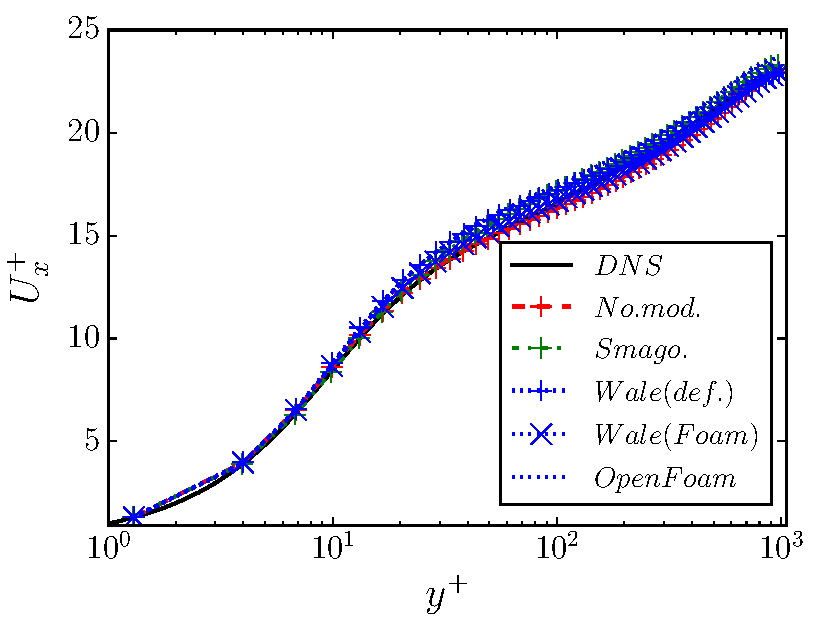
\includegraphics[width=0.5\textwidth]{./coarser/um.pdf} &
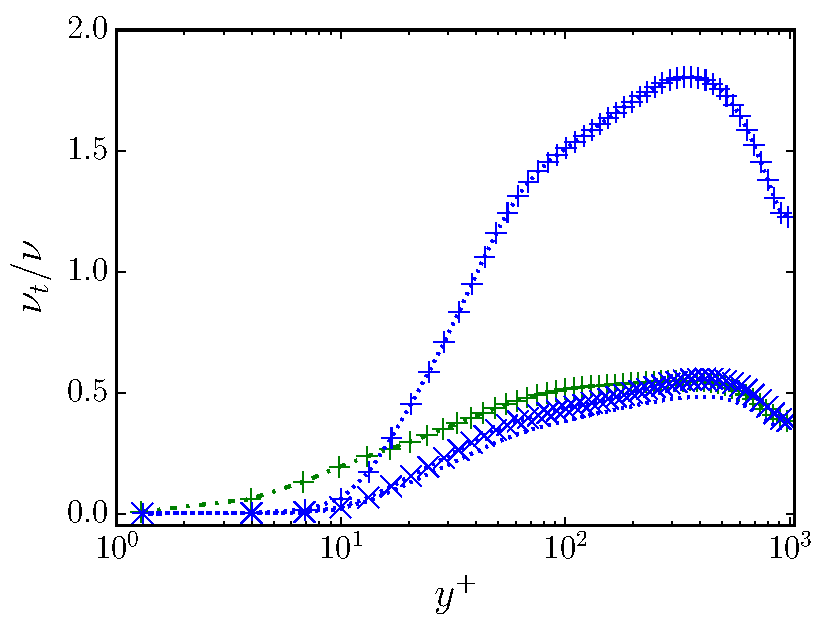
\includegraphics[width=0.5\textwidth]{./coarser/nu.pdf} \\
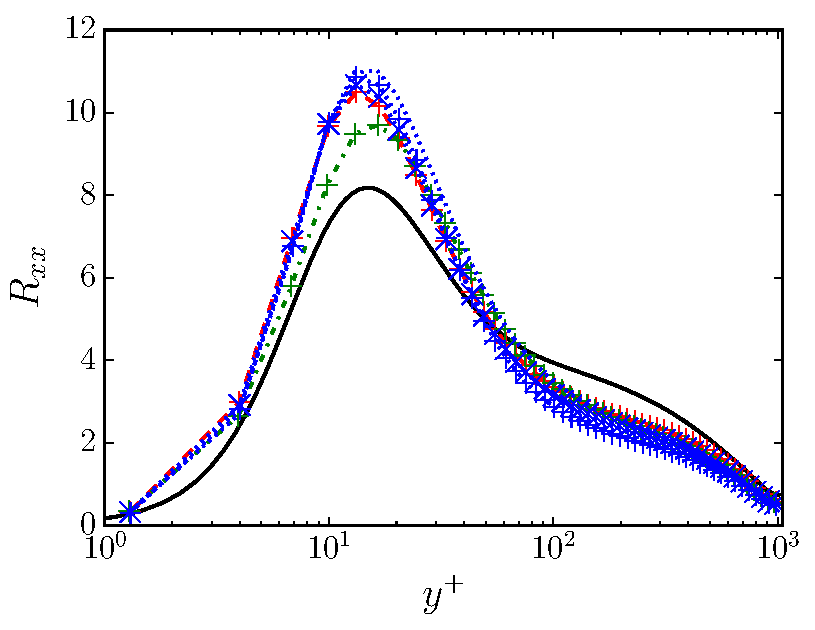
\includegraphics[width=0.5\textwidth]{./coarser/rxx.pdf} &
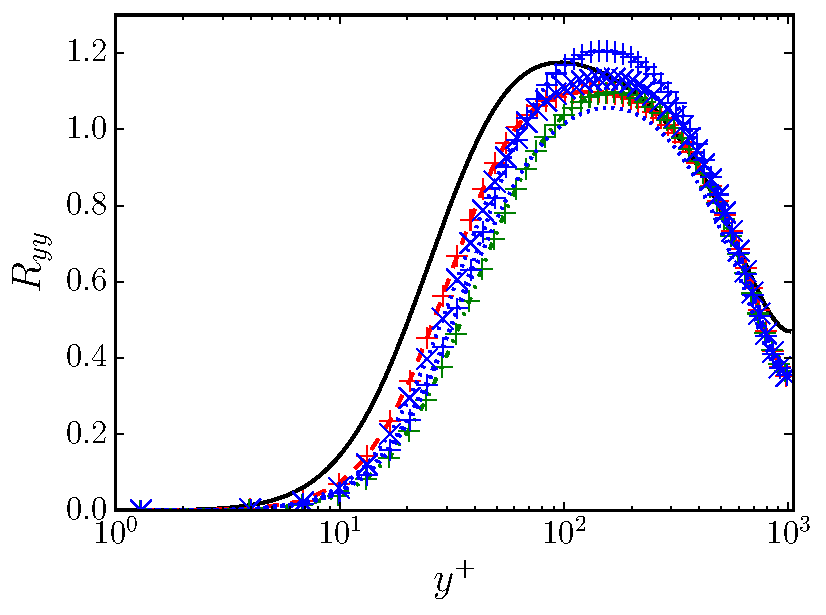
\includegraphics[width=0.5\textwidth]{./coarser/ryy.pdf} \\
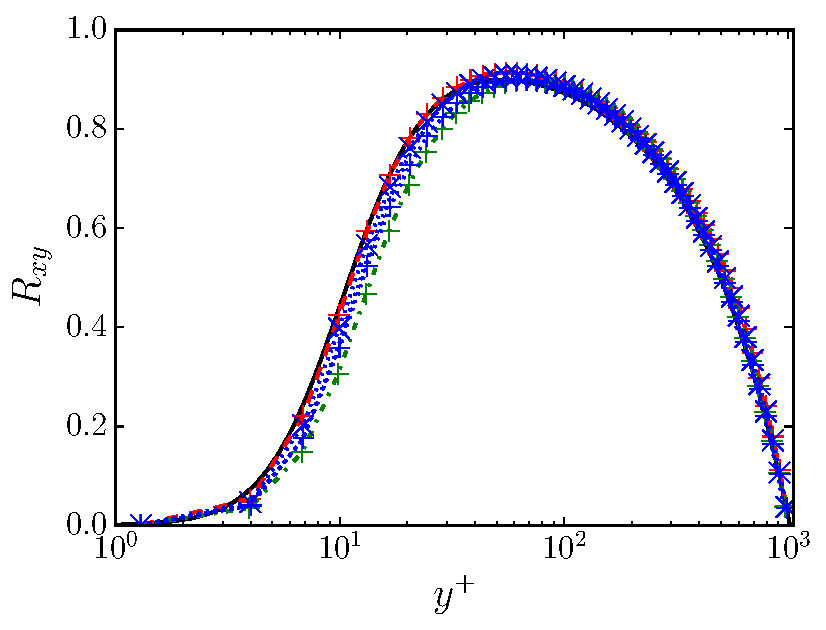
\includegraphics[width=0.5\textwidth]{./coarser/rxy.pdf} &
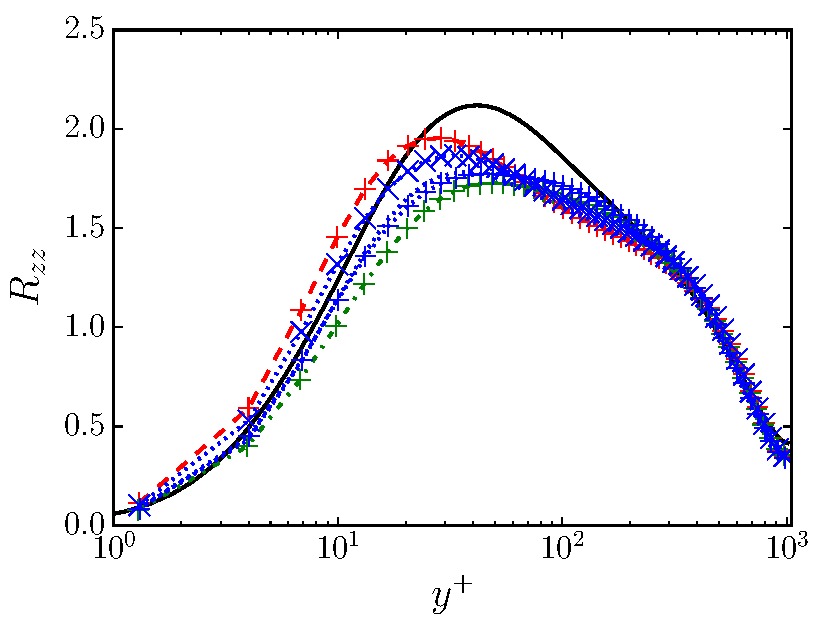
\includegraphics[width=0.5\textwidth]{./coarser/rzz.pdf} \\
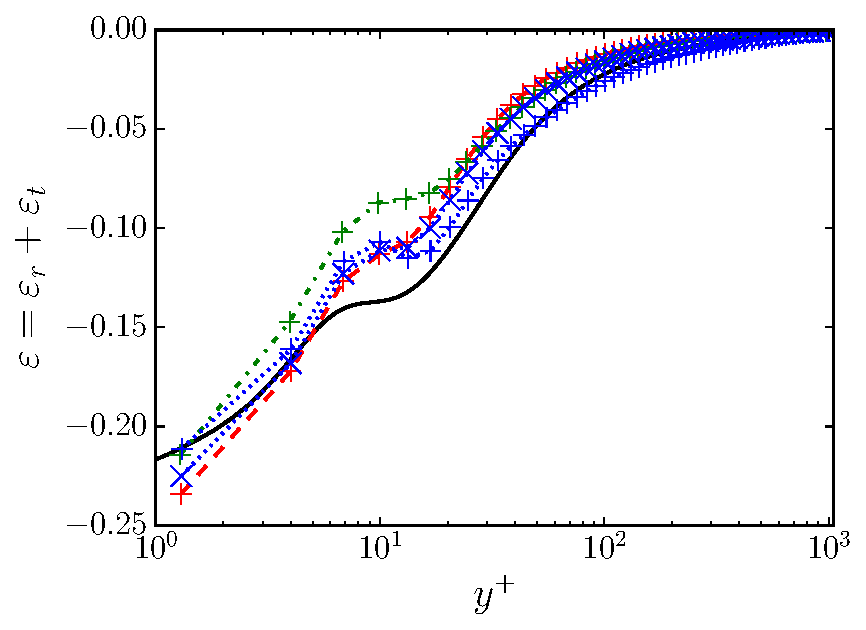
\includegraphics[width=0.5\textwidth]{./coarser/diss.pdf} &
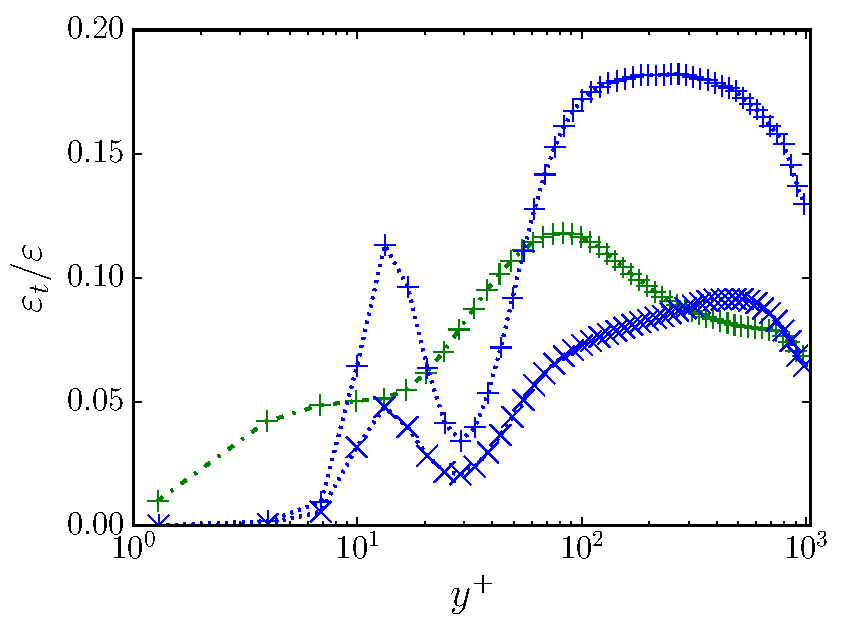
\includegraphics[width=0.5\textwidth]{./coarser/turb_diss.pdf}
\end{tabular}
\caption{Results on the coarser grid. Top-left: Averaged velocity. Top-right: Normalised turbulent viscosity. Middle: Reynolds stresses. Bottom-left: Total dissipation. Bottom-right: Turbulent dissipation.}
\label{fig-umnurij}
\end{figure}

\subsection{Finer grid}

On the finer grid, we are comparing the DNS with 7 simulations performed with \CS:
\begin{description}
\item[$No.Mod.$:] no SGS model
\item[$Smag.$:] Standard Smagorinsky model
\item[$Wale$:] default WALE model
\item[$Dyn.(def.)$:] default dynamic model ($-100 C_s^2 \leq C \leq 100 C_s^2$)
\item[$Dyn.(clip)$:] dynamic model with modified clipping: $0 \leq C \leq C_s^2$
\item[$Dyn.(def.)+<>$:] default dynamic model with spatial averaging in homogeneous directions as filtering operation ($-100 C_s^2 \leq C \leq 100 C_s^2$)
\item[$Dyn.(clip)+<>$:] dynamic model with spatial averaging in homogeneous directions as filtering operation and modified clipping: $0 \leq C \leq C_s^2$
\end{description}

For some of those simulations, we have obtained a reconstructed $C_s$, which is defined by analogy with the standard Smagorinsky model. The reconstructed $C_s$ is defined and approached by
\begin{eqnarray}
C_s^2 & = & \frac{\mu_t}{\rho \Delta^2 \sqrt{2 S_{ij} S_{ij}}} \nonumber \\
C_s & \approx & \sqrt{ \overline{ C_s^2 }} \nonumber
\end{eqnarray}
The reconstructed $C_s$ is an approximation of $\overline{C_s}$. It is a good one only when the RMS of $C_s$ is small compared to $\overline{C_s}$. To assess this, for one simulation, we have extracted the exact $\overline{C_s}$ and the associated RMS. On the whole domain, the amplitude of the RMS was around $60\%$ of $\overline{C_s}$. This leads to a reconstructed $C_s$ roughly $20\%$ higher when compared with the exact one. Based on this result, the reconstructed $C_s$ is not plotted here.

Figure \ref{fig-finer-umnu}, the averaged velocity and turbulent viscosity are plotted. The default dynamic model overestimate the averaged velocity, even when the filtering is replaced by spatial averaging in the homogeneous directions. As for the turbulent viscosity, the default dynamic model and the WALE model produce a similar one. For both quantities considered here, replacing the filter by a spatial average in the homogeneous directions has no visible impact.

\begin{figure}[htbp]
\begin{tabular}{c}
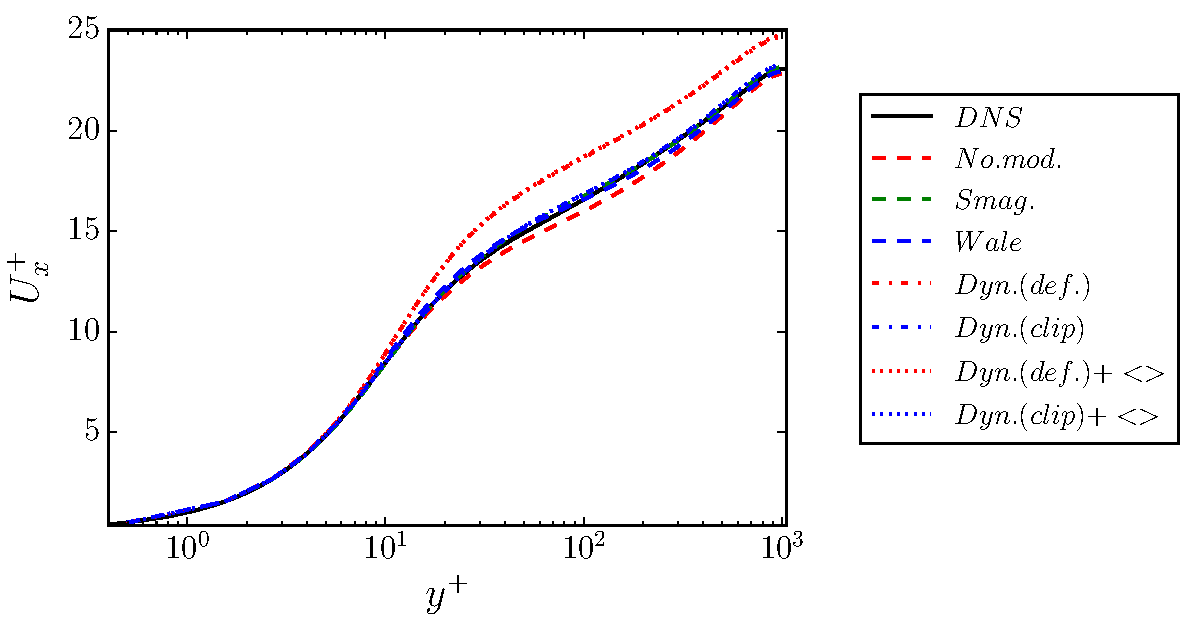
\includegraphics[width=\textwidth]{./finer/um.pdf} \\
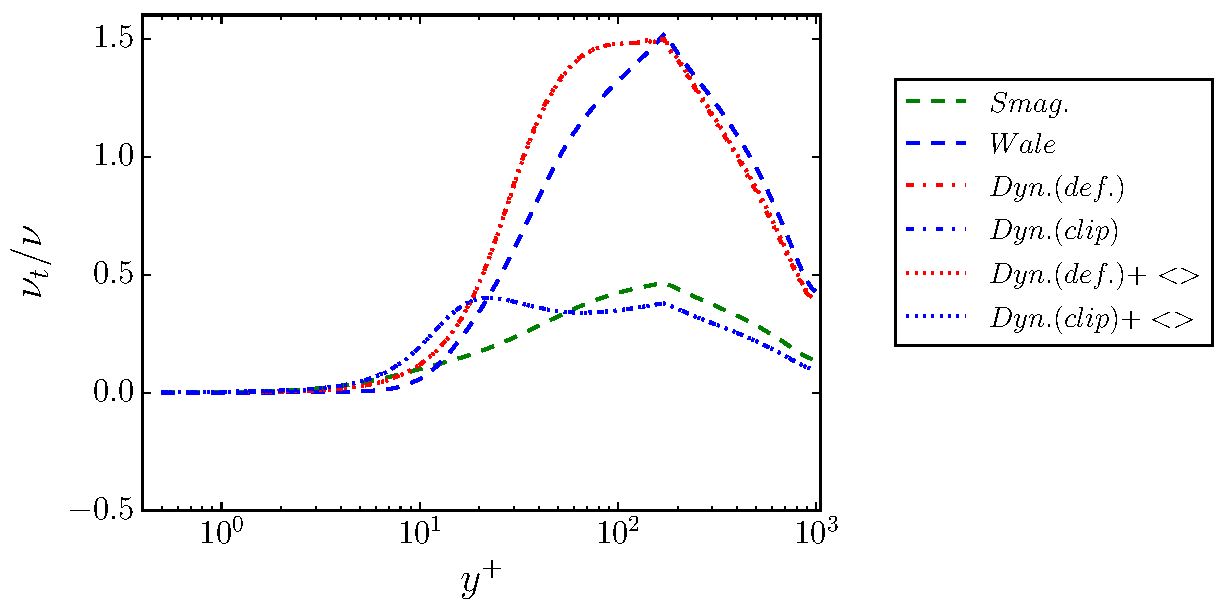
\includegraphics[width=\textwidth]{./finer/nu.pdf}
\end{tabular}
\caption{Results on the finer grid. Top: Averaged velocity. Bottom: Normalised turbulent viscosity.}
\label{fig-finer-umnu}
\end{figure}

Figure \ref{fig-finer-rij}, the Reynolds stresses are plotted. Both versions of the default dynamic model produce results that are not in good agreement with the DNS, especially for $R_{yy}$. The other models produce Reynolds stresses that are in a qualitative agreement when compared with DNS.

\begin{figure}[htbp]
\begin{tabular}{c}
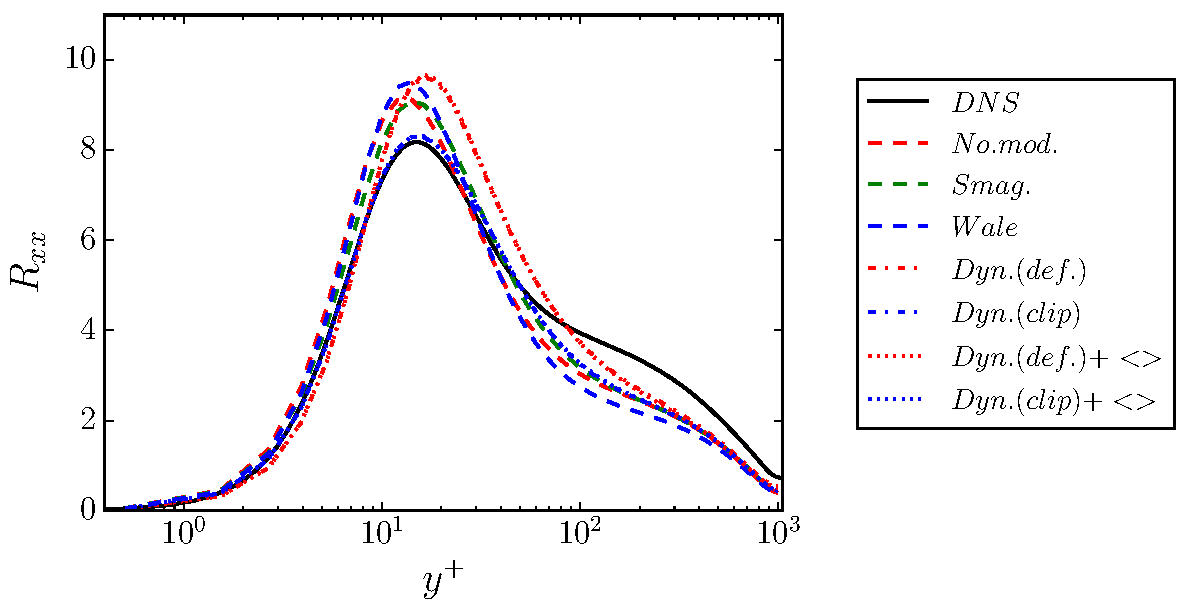
\includegraphics[width=0.8\textwidth]{./finer/rxx.pdf} \\
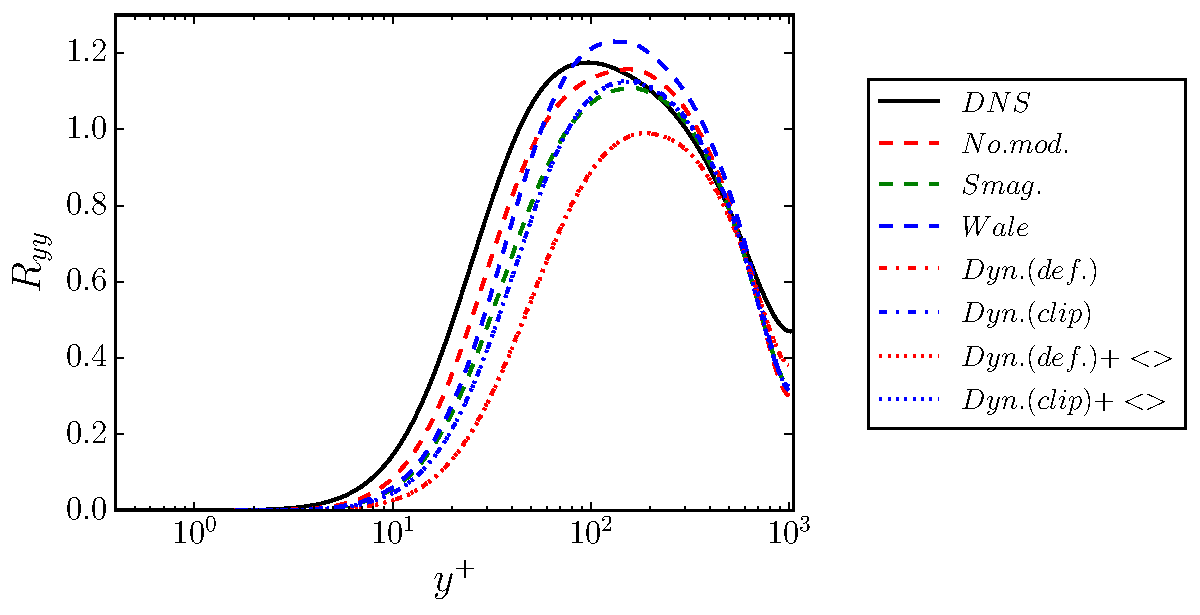
\includegraphics[width=0.8\textwidth]{./finer/ryy.pdf} \\
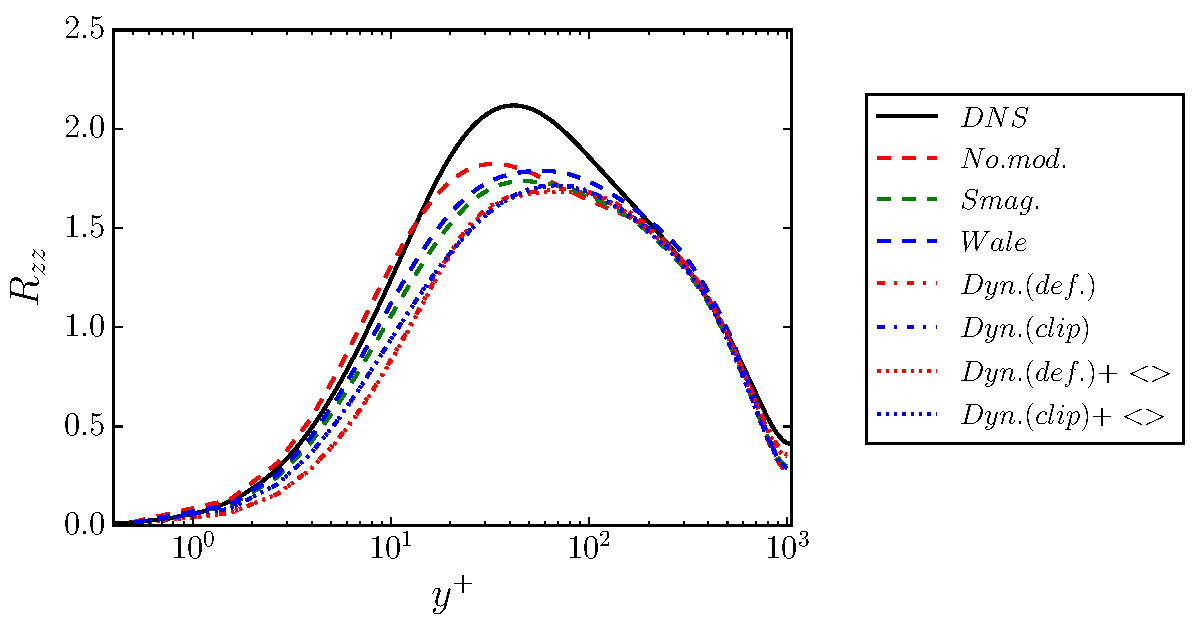
\includegraphics[width=0.8\textwidth]{./finer/rzz.pdf} \\
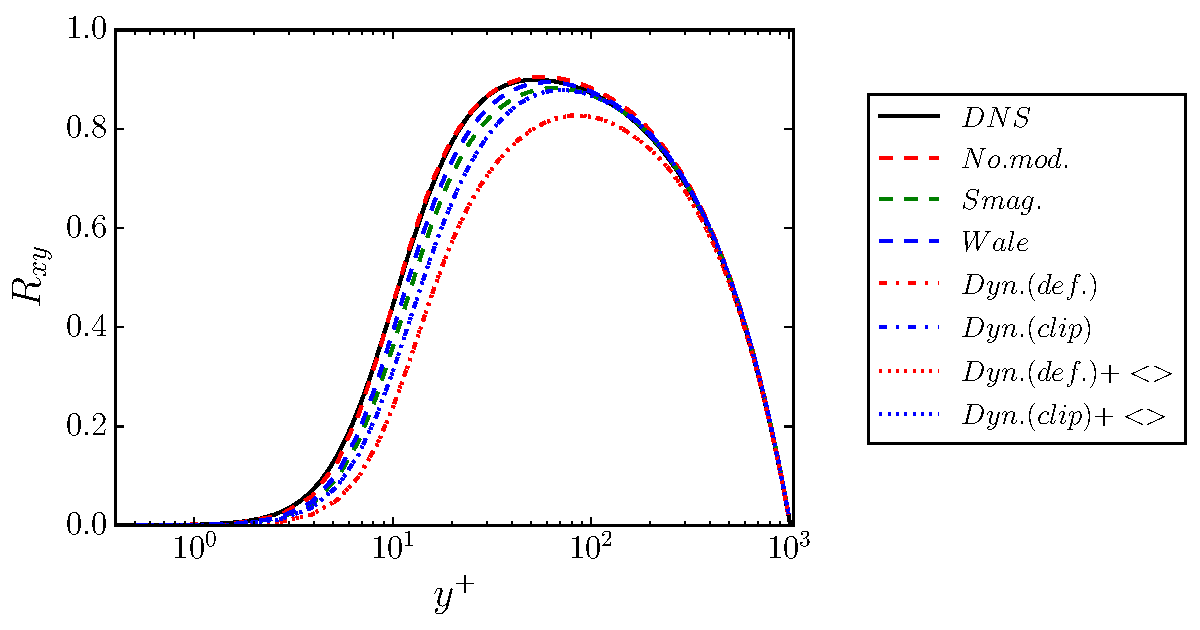
\includegraphics[width=0.8\textwidth]{./finer/rxy.pdf}
\end{tabular}
\caption{Results on the finer grid. Reynolds stresses.}
\label{fig-finer-rij}
\end{figure}

Figure \ref{fig-finer-diss}, %the reconstructed $C_s$, 
the dissipation rate and the turbulent dissipation are plotted. The dynamic models lead to an under-estimation of the dissipation. As far as the dissipation is concerned, the WALE model seems to perform slightly better compared with the others, although there are no huge differences between models.

\begin{figure}[htbp]
\begin{tabular}{c}
%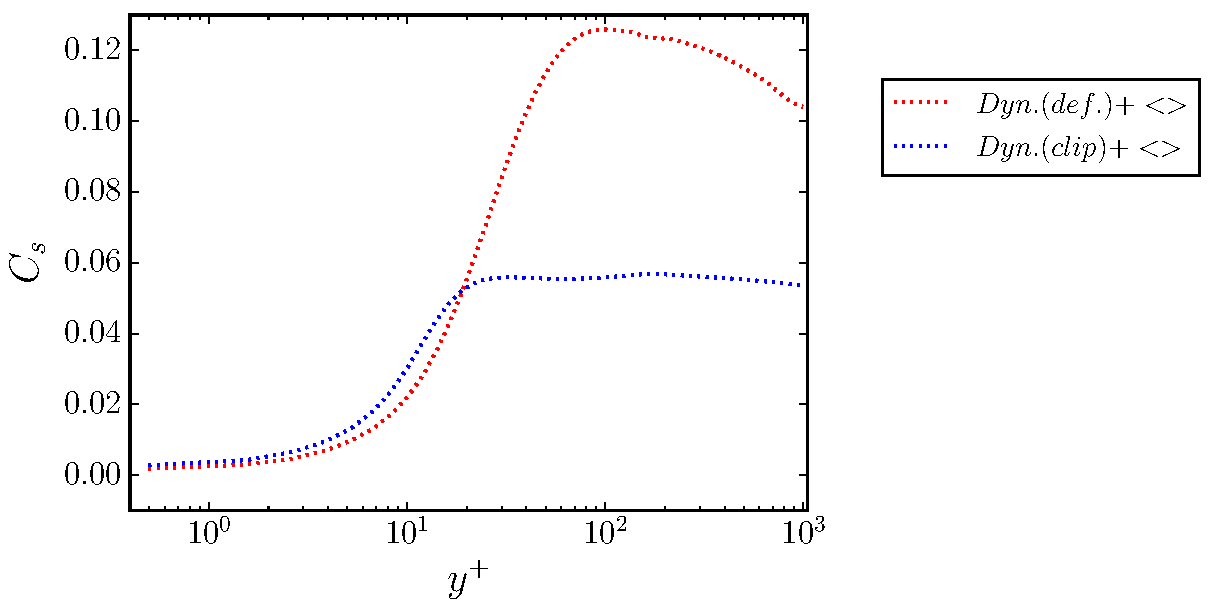
\includegraphics[width=\textwidth]{./finer/cs.pdf} \\
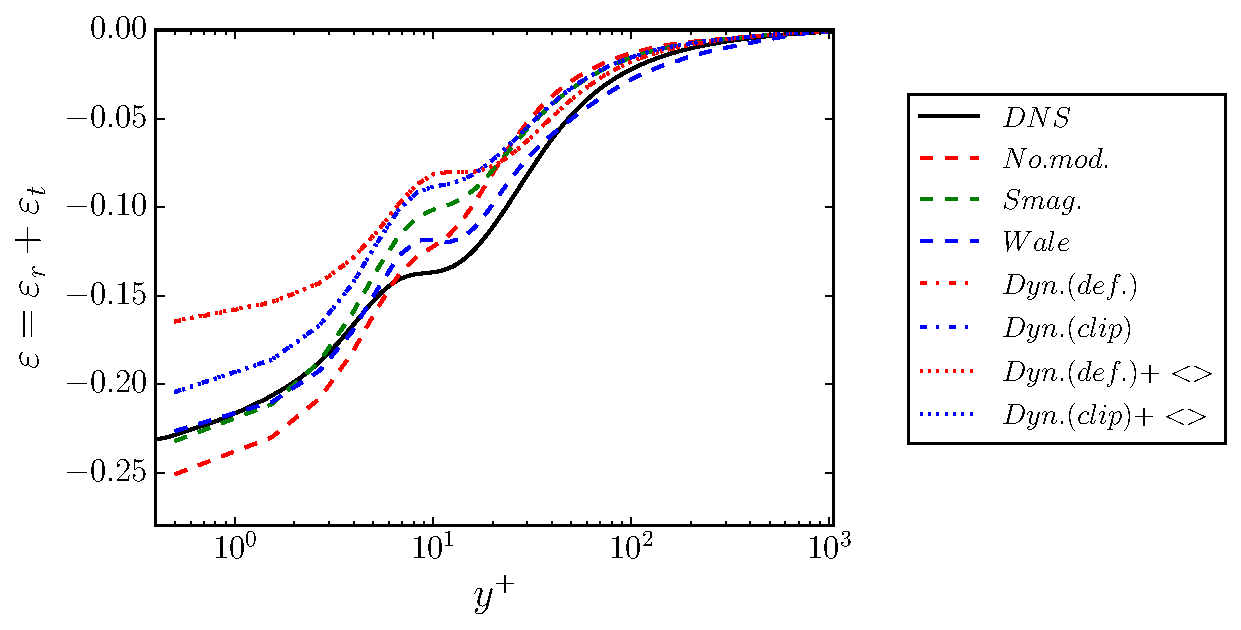
\includegraphics[width=\textwidth]{./finer/diss.pdf} \\
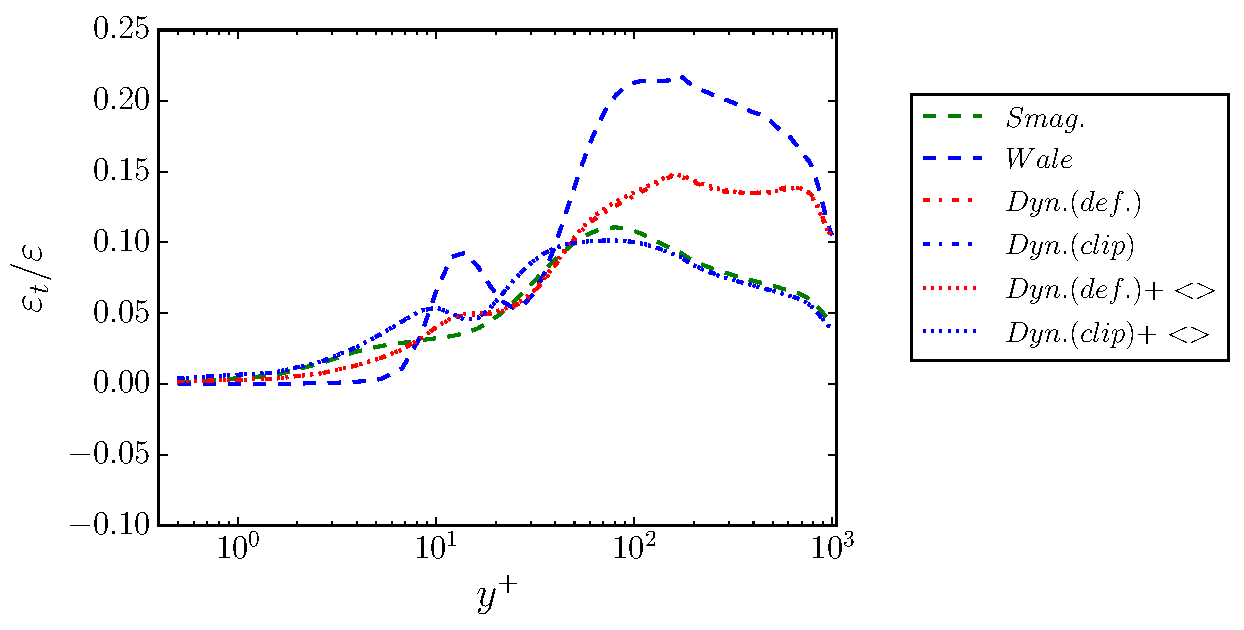
\includegraphics[width=\textwidth]{./finer/turb_diss.pdf}
\end{tabular}
\caption{Results on the finer grid. Top: %Reconstructed $C_s$. Middle: 
Total dissipation. Bottom: Turbulent dissipation.}
\label{fig-finer-diss}
\end{figure}

\clearpage

\appendix
\section{Gmsh script} \label{section_gmsh}
Below is the '.geo' script used to generate a 1D mesh for the lower half of the domain.
\begin{verbatim}
lx = 6.283;
lz = 3.142;
nx = 200.0;
nz = 200.0;

lc = 1e-7;
dx = lx / nx;
dz = lz / nz;

ypos = 0;
dy0 = 1 / 1020;
raison = 1.09;

p1 = newp;
Point(p1) = {0, -1, 0, lc};
autoPoint[] = Translate {dx, 0, 0} { Duplicata{ Point{p1}; } };
p2 = autoPoint[0];
autoPoint[] = Translate {0, 0, dz} { Duplicata{ Point{p1}; } };
p3 = autoPoint[0];
autoPoint[] = Translate {dx, 0, dz} { Duplicata{ Point{p1}; } };
p4 = autoPoint[0];
l1 = newl;
Line(l1) = {p1, p2};
l2 = newl;
Line(l2) = {p1, p3};
l3 = newl;
Line(l3) = {p4, p2};
l4 = newl;
Line(l4) = {p4, p3};
Transfinite Line {l1, l2, l3, l4} = 2 Using Progression 1;
l5 = newll;
Line Loop(l5) = {l1, -l3, l4, -l2} ;
s6 = news;
Plane Surface(s6) = {l5} ;
Transfinite Surface{s6};
Recombine Surface {s6};

dy = dy0;
For i In {0:32}

  autoVol[] = Extrude {0, dy, 0} { Surface{s6}; Layers{1}; Recombine; };

  ypos = ypos + dy;

  s6 = autoVol[5];
  Transfinite Surface{s6};
  Recombine Surface {s6};
  s6 = autoVol[4];
  Transfinite Surface{s6};
  Recombine Surface {s6};
  s6 = autoVol[3];
  Transfinite Surface{s6};
  Recombine Surface {s6};
  s6 = autoVol[2];
  Transfinite Surface{s6};
  Recombine Surface {s6};
  s6 = autoVol[0];
  Transfinite Surface{s6};
  Recombine Surface {s6};
  v6 = autoVol[1];
  Transfinite Volume{v6};

  dy *= raison;

EndFor


dy = (1-ypos)/53;
For i In {33:85}

  autoVol[] = Extrude {0, dy, 0} { Surface{s6}; Layers{1}; Recombine; };

  ypos = ypos + dy;

  s6 = autoVol[5];
  Transfinite Surface{s6};
  Recombine Surface {s6};
  s6 = autoVol[4];
  Transfinite Surface{s6};
  Recombine Surface {s6};
  s6 = autoVol[3];
  Transfinite Surface{s6};
  Recombine Surface {s6};
  s6 = autoVol[2];
  Transfinite Surface{s6};
  Recombine Surface {s6};
  s6 = autoVol[0];
  Transfinite Surface{s6};
  Recombine Surface {s6};
  v6 = autoVol[1];
  Transfinite Volume{v6};

EndFor
\end{verbatim}

%\begin{thebibliography}{9}
%
%\bibitem{abe2004surface}
%  Abe H., Kawamura H.and Matsuo Y.,
%  Surface heat-flux fluctuations in a turbulent channel flow up to $Re_\tau$= 1020 with $Pr$= 0.025 and 0.71,
%  \textit{International Journal of Heat and Fluid Flow},
%  Vol. 25,
%  Is. 3,
%  pages 404-419,
%  2004

%\end{thebibliography}
\end{document}